\documentclass{amsart}
\usepackage{amssymb}
\usepackage{amsmath}
\usepackage[latin1]{inputenc}

\usepackage{parskip}
\usepackage{float}
\usepackage{subfigure}

\usepackage{graphicx}

\usepackage{hyperref}
\hypersetup{colorlinks=true,
			urlcolor=cyan}
\def\N{\mathbb{N}}
\def\Z{\mathbb{Z}}
\def\Q{\mathbb{Q}}
\def\R{\mathbb{R}}
\def\C{\mathbb{C}}
\def\K{\mathbb{K}}

\def\diam{\mathrm{diam}}
\def\dom{\mathrm{dom}}
\def\card{\mathrm{card}}
\def\Re{\mathrm{Re}}
\def\Im{\mathrm{Im}}
\def\lin{\mathrm{lin}}
\def\dim{\mathrm{dim}}
\def\codim{\mathrm{codim}}
\def\co{\mathrm{co}}
\def\Int{\mathrm{Int}}

\usepackage{enumerate}

\usepackage{vmargin}
\setmargins{2.5cm}       % margen izquierdo
{1.5cm}                        % margen superior
{15.5cm}                      % anchura del texto
{23.42cm}                    % altura del texto
{10pt}                           % altura de los encabezados
{1cm}                           % espacio entre el texto y los encabezados
{0pt}                             % altura del pie de página
{2cm}                           % espacio entre el texto y el pie de página
\begin{document}

\begin{center}
\textbf{\Large Ejercicios de Geometría Discreta}

\bigskip

David Cabezas Berrido

\end{center}

\begin{center}
	\textbf{\large Tarea 1: Polígonos}
\end{center}

\bigskip

\textbf{Ejercicio:} Prueba que el número de triangulaciones de un polígono de $n+2$ vértices está entre 1 y $C_n$.

\bigskip

\textbf{Soluci\'on:} Hemos visto que todo polígono se puede triangular, luego la cota inferior está asegurada. Si el polígono fuese convexo se pueden trazar diagonales entre cada dos vértices no consecutivos, y ya sabemos que el número de triangulaciones es $C_n$. En caso de no ser convexo, la cantidad de diagonales que se pueden trazar es estrictamente menor, luego el número de triangulaciones diferentes no puede aumentar.

\bigskip

\textbf{Ejercicio:} Para cada $n > 3$ encuentra polígonos de $n$ vértices con
exactamente 2 triangulaciones.

\bigskip

\textbf{Solución:} Para $n=4$, podemos tomar simplemente un rectángulo, que es convexo y tiene $C_2=\frac{1}{3}\binom{4}{2}=2$ triangulaciones. Para $n\geq 5$, podemos colocar todos los vértices menos dos en una media luna como indican los puntos azules del dibujo y unimos cada uno con el siguiente obteniendo una poligonal abierta. A continuación, colocamos un vértice (el rojo del dibujo) de tal forma que sólo ``vea'' a los tres primeros vértices azules, en el sentido de que no pueda unirse con los demás por una línea recta que no corte a las aristas ya colocadas entre los puntos azules. Trazamos una arista entre el nuevo vértice y el primer vértice azul, continuando nuestra curva poligonal abierta. Por último, colocamos el vértice restante (verde) de forma que vea a todos los vértices ya colocados excepto al vértice azul que unimos con el rojo. Unimos el vértice verde con el rojo y cerramos el polígono añadiendo la arista entre el vértice verde y el último vértice azul.

\begin{figure}[H]
	\centering
	\subfigure[$n=4$]{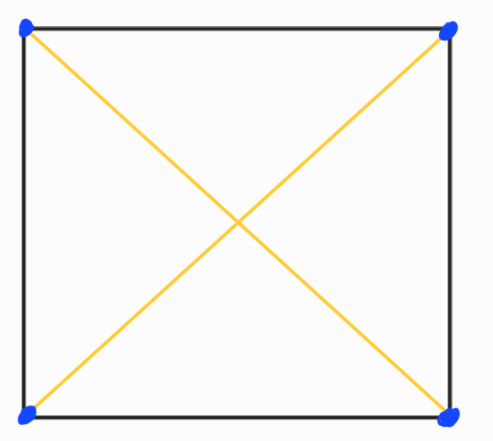
\includegraphics[width=60mm]{imgs/dostriang-4}}
	\subfigure[$n\geq 5$]{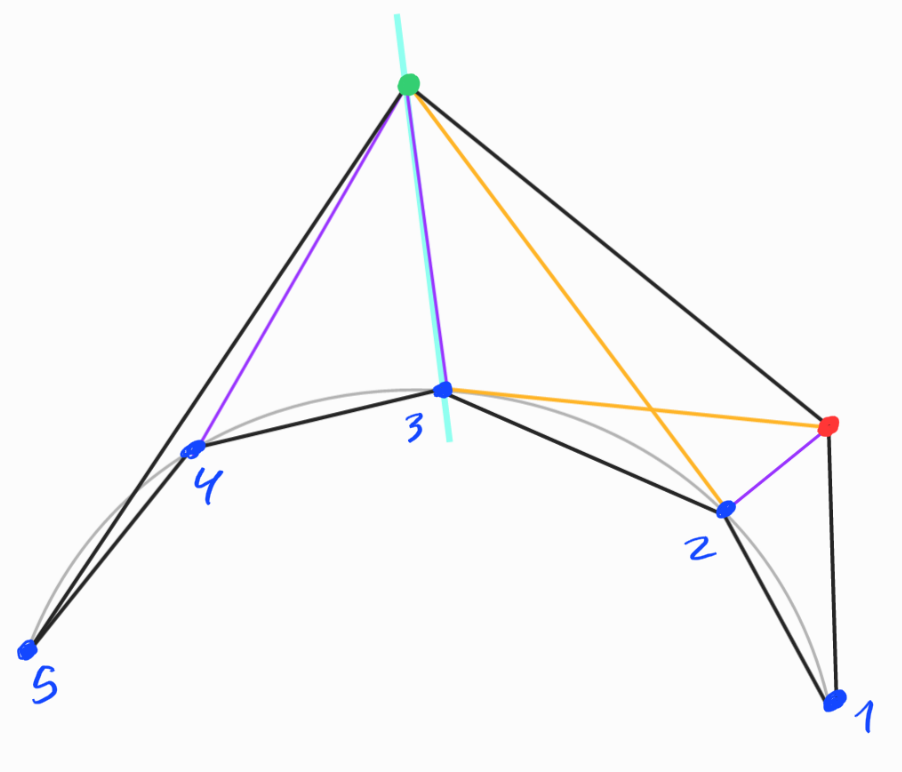
\includegraphics[width=70mm]{imgs/dostriang-5}}
\end{figure}

De esta forma, cada uno de los vértices azules (a excepción de los tres primeros y el último, que está unido con él) sólo ``ve'' al vértice verde, y a la hora de triangular el polígono la diagonal entre ese vértice azul y el verde es obligada. El primero y el último de los vértices azules están obligados a pertenecer a una oreja cada uno, puesto que sólo pueden unirse con los que ya comparten una arista. La diagonal que une el tercer vértice azul con el verde también es obligada para cerrar el triángulo que queda a un lado de la diagonal que une el cuarto vértice azul con el verde, a menos que sólo haya 3 vértices azules y ya estén unidos el 3º azul y el verde por una arista. Además, la oreja que contiene al primer vértice azul debe cerrarse con una diagonal entre el vértice rojo y el segundo azul, ya que el vértice 1 no puede unirse con el verde por dentro del polígono.  La conclusión de este razonamiento es que las diagonales en morado son obligadas.

Por la construcción que hemos hecho, para finalizar la triangulación hay únicamente dos posibilidades, las dos líneas amarillas del dibujo. Por tanto, hay sólo dos triangulaciones posibles.

Aunque en el dibujo hayamos puesto 7 vértices, se puede hacer para cualquier número mayor o igual a 5 simplemente cambiando el número de vértices azules que ponemos en la media luna (mínimo 3). Por ejemplo, para $n=5$ podemos cortar el polígono del dibujo por la línea cian y quedarnos con el polígono de la derecha.

\bigskip

\textbf{Ejercicio:} Para cada $n \geq 3$  prueba que no existen polígonos de $n + 2$
vértices con exactamente $C_n - 1$ triangulaciones.

\bigskip

\textbf{Solución:} Consideremos un polígono de $n+2$ vértices, que como mínimo serán 5. Si el polígono es convexo tendrá $C_n$ triangulaciones, luego supondremos que no lo es. Existe un vértice no estrictamente convexo, luego no se puede trazar una diagonal entre sus adyacences y el vértice no puede formar parte de una oreja. Por tanto, habrá que unir el vértice con otro forzosamente. ?ara ello tenemos como máximo $n-1$ opciones posibles, puesto que no se puede unir ni con él mismo ni con los adyacentes. En el mejor de los casos hay $n-1$ opciones, y para cada una de ellas dividiríamos el polígono en dos por esa diagonal. Los dos polinomios resultantes suman $n+4$ vértices debido a que estamos contando dos veces los vértices por los que pasa la diagonal, y se pueden triangular de forma independiente. El número de triangulaciones de cada uno será menor o igual a $C_{k-2}$ y $C_{l-2}$ donde $k+l=n+4$ y $3\leq k,l\leq n+1$ (los vértices adyacentes al vértice por el que trazamos la diagonal quedan cada uno en un polígono diferente). Por tanto, el número de triangulaciones del polígono estará acotado por
\[\sum_{k=3}^{n+1} C_{k-2} C_{n-k+2}=\sum_{k=1}^{n-1} C_{k} C_{n-k}.\]
Es conocido que los números de Catalan verifican $C_0=1$ y 
$C_n=\sum\limits_{k=0}^n C_k C_{n-k}$,
luego el número de triangulaciones es menor o igual que $C_n-2$ (hay dos términos menos y todos los sumandos son mayores o iguales que 1).

\bigskip

\textbf{Ejercicio:} Prueba que todo polígono con $r$ agujeros se puede triangular
por diagonales y deduce cuál será el número de triángulos y de
diagonales de una triangulación cualquiera en función de sus
vértices y agujeros.

\bigskip

\textbf{Solución:} Primero razonaremos que es posible triangularlo. Haremos inducción en el número de agujeros, ya sabemos que se cumple para $r=0$. Supongamos que cualquier polígono con un número de agujeros menor que $r>0$ se puede triangular, y consideremos un polígono con $r$ agujeros.

Fijemos cualquier orientación que haga que el polígono (agujeros incluídos) no tenga aristas horizontales ni verticales y de forma que no haya dos vértices en la misma vertical ni horizontal. Esto es posible porque el número de vértices y aristas es finito. Fijémonos en uno de los agujeros ($A$ en el dibujo). Tomemos el vértice más al oeste (1), y sus dos vértices adyacentes (2 y 4). Desplazamos una recta vertical desde 1 hacia la izquierda hasta chocar con un vértice que se pueda unir con 1 (5 en el dibujo), éste no pertenecerá al agujero puesto que 1 es el más al oeste. Siempre llegamos a un vértice que se puede unir con 1, ya que siempre chocamos con al menos dos aristas del polígono exterior y al final de ellas habrá un vértice, si alguna arista se entromete entre 1 y el vértice, acabaremos chocando con su extremo a menos que otra arista nos tape, pero entonces chocaremos con el extremo de la nueva arista \ldots \ y así hasta que toquemos un vértice, la cantidad finita de aristas lo garantiza. Si hemos acabado en el polígono exterior paramos (es el caso del dibujo), si hemos acabado en otro agujero hacemos lo mismo con el vértice más a la izquierda de ese agujero. De esta forma siempre acabamos en un vértice del polígono exterior.

\begin{figure}[H]
	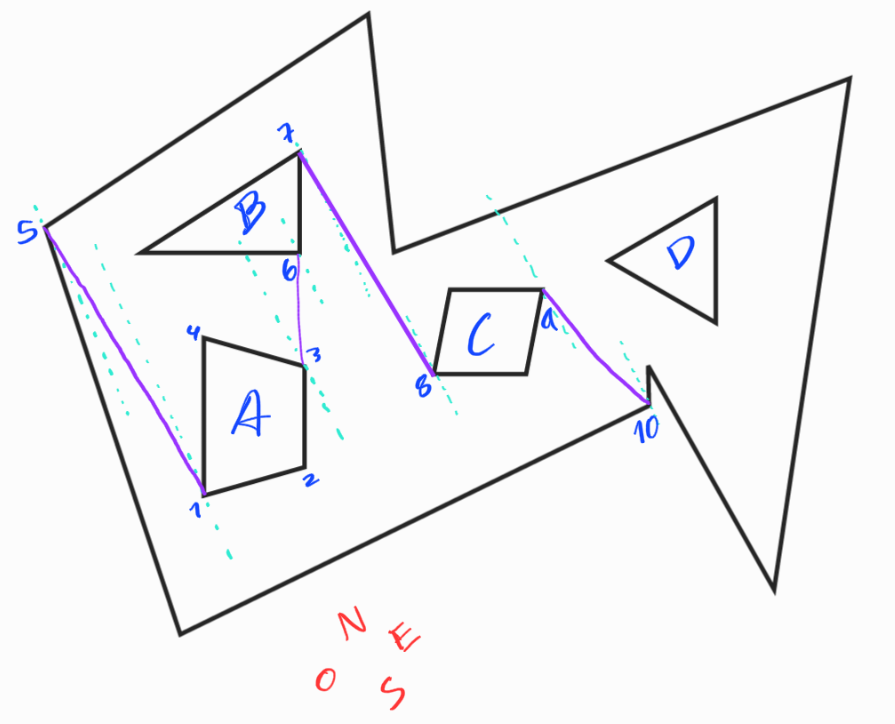
\includegraphics[width=100mm]{imgs/triang-agujeros}
\end{figure}

Ahora repetimos el proceso con el vértice más a la derecha (3) del agujero $A$ que tomamos inicialmente. En este caso, saltamos al agujero $B$ (vértice 6) y salimos por el vértice 7, nos vamos al vértice 8 (agujero C), salimos por el 9 y llegamos al 10, que pertenece al polígono exterior. Los vértices 5 y 10 no podrían ser el mismo, puesto que el 5 está al oeste de 1 (el más al oeste del agujero $A$) y 10 está al este de 3 (el más al este del agujero $A$). Al hacer esto, hemos partido el polígono original en dos polígonos (norte y sur) con menos agujeros, ya que tenemos garantizado que $A$ separa ambos polígonos. Tanto el polígono norte como el sur se pueden triangular por la hipótesis de inducción, y añadiendo las diagonales que hemos colocado, queda triangulado el polígono original.

Ahora usaremos los ángulos para deducir el número de triángulos y diagonales de una triangulación cualquiera. Sea un polígono $P$ con $n$ vértices y $k$ agujeros $P_1,\ldots, P_k$ cada uno con $n_k$ vértices. Sabemos que la suma de los ángulos interiores de $P$ (sin contar los agujeros) es $(n-2)\pi$ y la de los exteriores $(n+2)\pi$, y lo mismo ocurre con $(n_k-2)\pi$ y $(n_k+2)\pi$ para cada agujero. Los ángulos exteriores de los agujeros son ángulos interiores para $P$, luego los ángulos interiores de $P$ suman

\begin{align*}
(n-2)\pi+\sum_{j=1}^k (n_k+2)\pi&=\pi\left(n-2+\sum_{j=1}^k (n_k+2)\right)=\pi\left(n-2+\sum_{j=1}^k n_k+2k\right)\\&=\pi\left(n+\sum_{j=1}^k n_k+2(k-1)\right)
\end{align*}

Una triangulación de $P$ estará formada por triángulos en el interior de $P$ exterior de los agujeros, luego la suma de los ángulos de los triángulos será la suma de los ángulos interiores de $P$, como la suma de los ángulos de cada uno es $\pi$, habrá exactamente $n+\sum\limits_{j=1}^k n_k+2(k-1)$. triángulos. Para las diagonales, si tenemos $T$ triángulos, por separado tendremos $3T$ lados. Si quitamos las aristas del polígono (tanto interiores como exteriores) nos quedarán las diagonales, pero debemos dividir esta cantidad por dos, puesto que cada diagonal es compartida por dos triangulos y la estamos contando dos veces. Por tanto, el número de diagonales será al mitad de 

\[3\left(n+\sum_{j=1}^k n_k+2(k-1)\right)-\left(n+\sum_{j=1}^k n_k\right)=2\left(n+\sum_{j=1}^k n_k\right)+6(k-1),\]
es decir,
\[n+\sum_{j=1}^k n_k+3(k-1).\]

\bigskip

\begin{center}
	\textbf{\large Tarea 2: Galería de Arte}
\end{center}

\bigskip

\textbf{O'Rourke y Wood, 1983:} $E^+[n/2]$ V-guardias son necesarios y suficientes para ver el exterior de un polígono de $n$ lados.

\bigskip

\textbf{Demostración:} Sea $P$ un polígono cualquiera con $n$ lados. Comenzamos haciendo su envolvente convexa y triangulando la parte de su envolvente convexa exterior a $P$, esto nos genera un grafo plano $G''$.

\begin{figure}[H]
	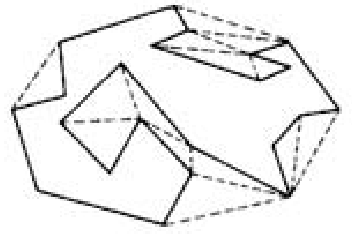
\includegraphics[width=70mm]{imgs/museo-g2}
\end{figure}

Ahora añadimos un nuevo vértice $V_\infty$ en el exterior del grafo y lo conectamos a los vértices de la envolvente convexa, es decir, los que dan al exterior de $G''$. Así obtenemos un nuevo grafo (plano) $G'$. Las nuevas aristas rodearán a $G''$ por arriba o por abajo (o izquierda y derecha, según donde coloquemos $V_\infty$) hasta llegar a cada vértice. El último vértice que rodeemos por cada lado no quedará ``encerrado'' por las nuevas aristas (el resto sí). Llamaremos $x$ a uno de los dos vértices que todavía dan al exterior del grafo a parte de $V_\infty$.

\begin{figure}[H]
	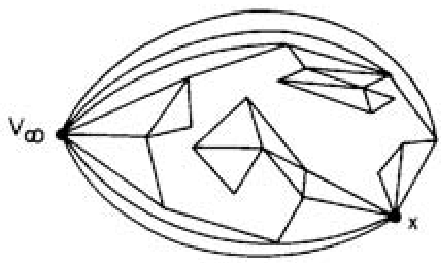
\includegraphics[width=80mm]{imgs/museo-g1}
\end{figure}

Ahora abrimos el grafo duplicando el vértice $x$ en $x'$ y $x''$, ambos quedarán conectados con todos los vértices que lo estaban con $x$, conectaremos $V_\infty$ con $x'$ y $x''$ rodeando el grafo por dos lados  diferentes (arriba y abajo o izquierda y derecha). Obtenemos así el grafo $G$, que tiene $n+2$ vértices (hemos añadido $V_\infty$ y duplicado $x$).

\begin{figure}[H]
	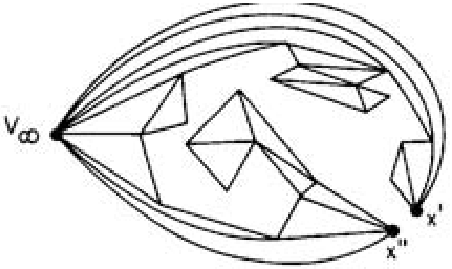
\includegraphics[width=80mm]{imgs/museo-g}
\end{figure}

 $G$ que es la triangulación de un polígono (al menos topológicamente hablando) y por tanto 3-coloreable. Coloreamos $G$ con los colores rojo, verde y azul, pongamos que $V_\infty$ queda rojo. Habrá un color que no esté presente en menos de $E[\frac{n+2}{3}]$ vértices. Si ese color no es el rojo, TODO

\bigskip

\begin{center}
	\textbf{\large Tarea 3: Equidescomposición de Polígonos}
\end{center}

\bigskip

\textbf{Ejercicio:} Encuentra otra descomposición poligonal de la cruz griega
que sea también descomposición de un cuadrado.

\bigskip

\textbf{Solución:} Presentamos la siguiente descomposición de la cruz, las piezas se organizan como en la imagen de la derecha para formar un cuadrado.

\begin{figure}[H]
	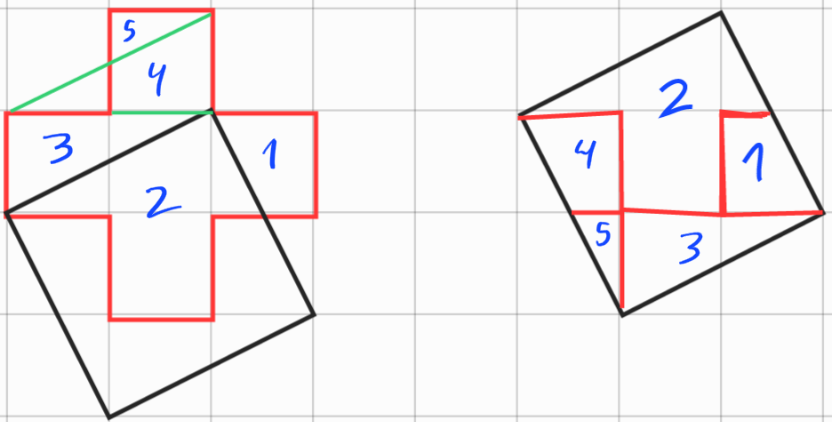
\includegraphics[width=100mm]{imgs/cruz-cuadrado}
\end{figure}

La pieza 2 queda en la misma posición. Como la diagonal secciona por la mitad el rectángulo de anchura 1 y altura 2 de la derecha (el que tiene el 1 arriba), la pieza 1 encaja en el hueco que queda abajo a la derecha de la 2. El mismo razonamiento hace que las piezas 4 y 5 encajen a la izquierda de la 2 (la 4) y debajo (la 5 debajo de la 4). El hueco que queda es exactamente medio rectángulo de altura 1 y anchura 2, donde encaja perfectamente la pieza 3. También es importante la orientación de las piezas, por ejemplo la sección verde que separa la 4 de la 5 debe darse seccionando por una recta con pendiente hacia arriba, si seccionamos con una recta de pendiente hacia abajo las piezas 4 y 5 no encajan (habría que reflejarlas).

\bigskip

\textbf{Ejercicio:} Encuentra descomposiciones poligonales de dos cruces griegas
que combinadas den una de un solo cuadrado.

\bigskip

\textbf{Solución:} Si ambas son del mismo tamaño, cada una se puede dividir fácilmente en 5 cuadrados iguales, y ya conocemos cómo 10 cuadrados iguales se descomponen en otro más grande (diapositiva 7).

\begin{figure}[H]
	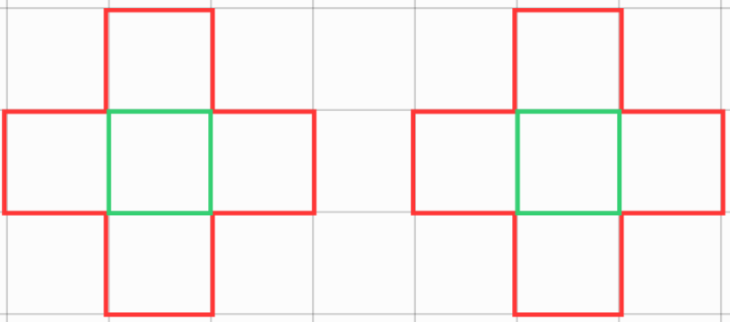
\includegraphics[width=80mm]{imgs/cruces-cuadrado1}
\end{figure}

Si una es exactamente el doble de grande de la otra, en la diapositiva 8 tenemos otra descomposición más.

También para el mismo tamaño, seccionando cada cruz por la mitad y pegándo las piezas como se indica en el dibujo es claro que se obtiene un cuadrado.

\begin{figure}[H]
	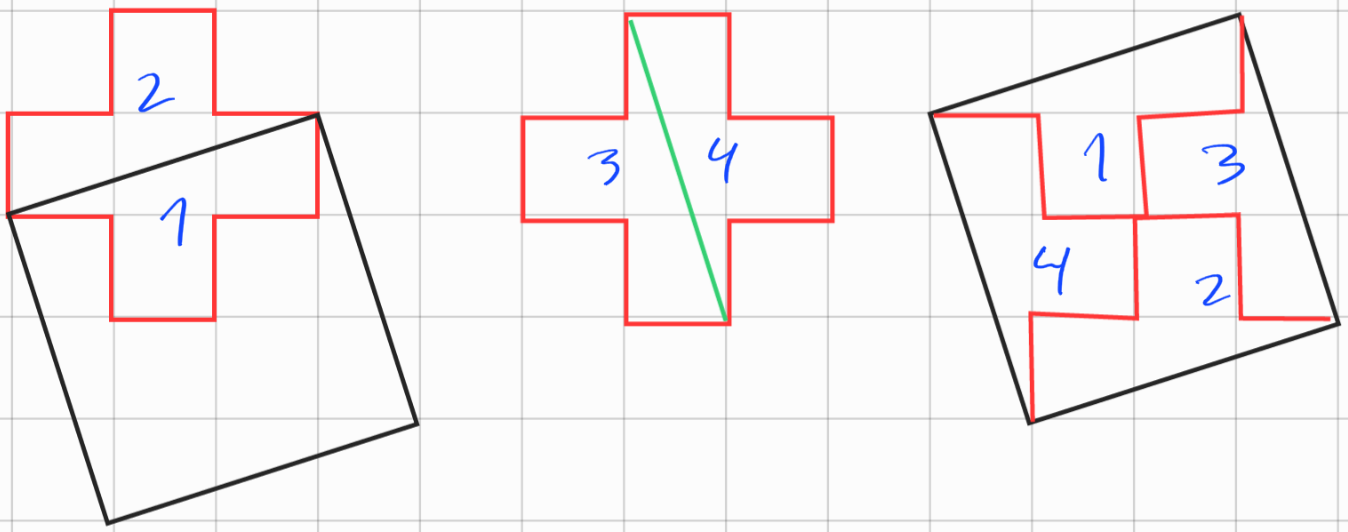
\includegraphics[width=100mm]{imgs/cruces-cuadrado2}
\end{figure}

\bigskip

\textbf{Ejercicio:} Encuentra una descomposición poligonal con tres elementos
de un triángulo que dé también una descomposición de su
imagen especular.

\bigskip

\textbf{Solución:} Dado un triángulo cualquiera, nos tomamos el lado más largo (si hay empate podemos coger un lado cualquiera) de forma que tenemos garantizado que la perpendicular por el vértice opuesto (altura) corte a ese lado. En el dibujo tomamos el lado negro de abajo. Trazamos la altura desde el vértice opuesto (en azul) y una paralela al lado que pase por el punto medio de la altura (también en azul), esta paralela también pasará por los puntos medios de los lados menores.

Ahora damos dos cortes (en morado), ambos desde el punto donde la altura corta al lado largo y cada uno hasta el punto medio de un lado menor (el punto amarillo donde la paralela azul corta al lado). Esto divide el triangulo en un cuadrilátero y dos triángulos pequeños (1 y 2). Trazamos otra paralela más al lado largo por el vértice opuesto (en verde) y prolongamos (en rojo) los cortes morados hasta que corten a dicha paralela. Como es paralela, tenemos garantizado que cada uno de los ángulos $\alpha$, $\beta$, $\gamma$ y $\delta$ se repite arriba tal como indica el dibujo en amarillo. Por tanto, el las piezas triangulares 1 y 2 que hemos separado al hacer los cortes morados encajan en las posiciones 1 y 2 rojas que hay entre la paralela azul y la paralela verde. Obtenemos así el triángulo reflejado.

\begin{figure}[H]
	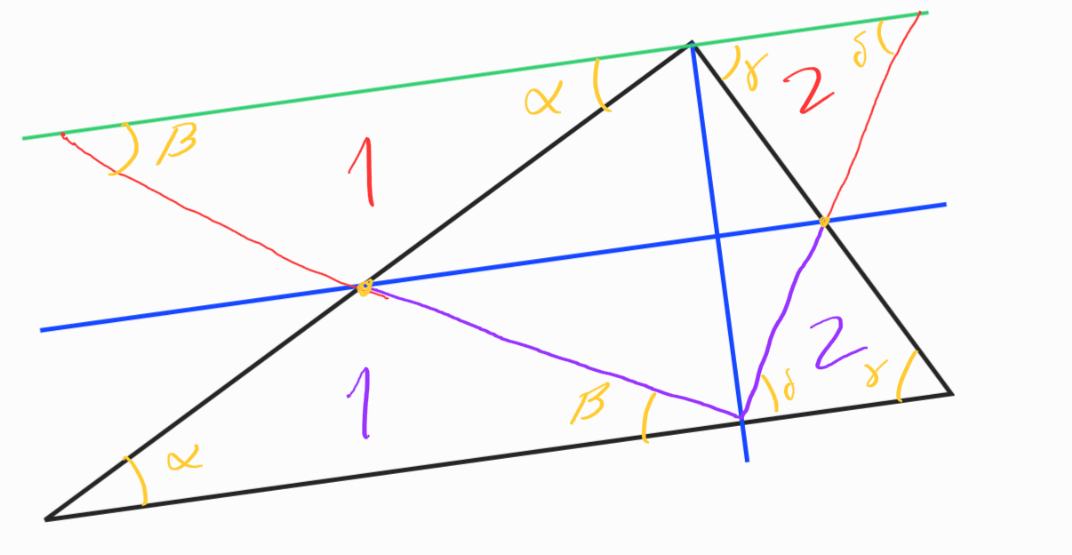
\includegraphics[width=100mm]{imgs/reflejar-triangulo}
\end{figure}


\bigskip

\textbf{Ejercicio:} Se puede asegurar que en un polígono dado, el número de
triángulos de una triangulación es menor o igual que el de una
descomposición por triángulos.

\bigskip

\textbf{Solución:} Claramente una triangulación es una descomposición por triángulos, luego TODO

TODO: El enunciado está muy mal redactado, ¿no? Preguntar

\bigskip
\begin{center}
	\textbf{\large Tarea 4: Equidescomposición de Poliedros}
\end{center}
\bigskip

\textbf{Ejercicio:} Encuentra los ángulos diedrales de un cubo, un tetraedro y un octaedro
regular. Prueba que el cubo no es equidescomponible con el tetraedro regular
del mismo volumen.

\bigskip

\textbf{Solución:} El de un cubo es claramente $\pi/2$. Como todas las aristas son perpendiculares entre sí, el ángulo entre dos caras cualesquiera es el ángulo que forman dos aristas en un vértice donde se corten.

Con el siguiente dibujo en mente, vemos que el ángulo diedral del tetraedro puede obtenerse a partir del triángulo rectangulo que tiene como hipotenusa la altura de una cara (triángulo equilátero), como cateto opuesto la altura del tetraedro y como cateto contiguo la apotema de una cara. Para facilitar los cálculos, podemos suponer (el ángulo no cambia por dilataciones) que la altura de los triángulos que forman las caras vale 1.

\begin{figure}[H]
	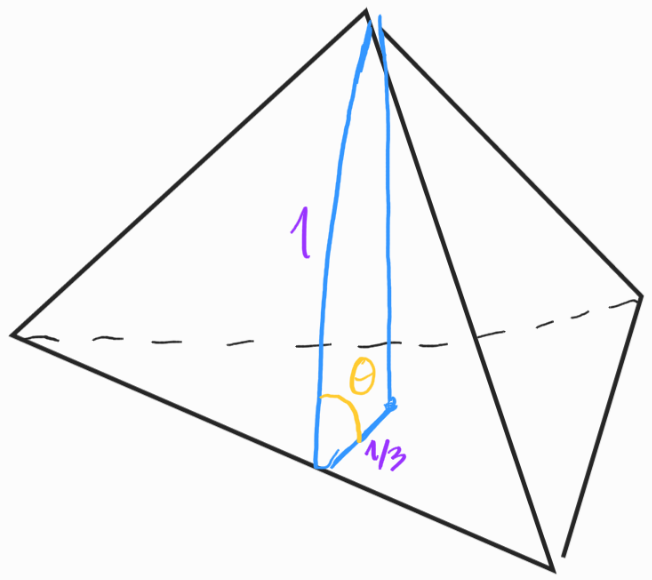
\includegraphics[width=80mm]{imgs/diedral-tetraedro}
\end{figure}

El lado contiguo al ángulo diedral es justamente la apotema del triángulo que forma la base del tetraedro. Sabemos que la apotema de un triángulo equilátero es un tercio de la altura, en este caso será $1/3$. Como la hipotenusa (la altura de una cara) vale 1, podemos obtener el ángulo como el arco coseno de $1/3$.

Para el octaedro el ángulo diedral será el doble de el que representamos en amarillo en la figura. Tenemos un triángulo rectángulo donde la hipotenusa es la altura de una cara y el cateto contiguo es la apotema de un cuadrado de lado igual al lado de los triángulos que forman las caras. Ahora, por simplicidad, supondremos que el lado de los triángulos equiláteros (las caras) mide 1. La altura de una cara será entonces $\sqrt{3}/2$, y la apotema del cuadrado será la mitad del lado, $1/2$. Por tanto, el ángulo representado en el dibujo será el arco coseno de $\frac{1/2}{\sqrt{3}/2}=1/\sqrt{3}$, y el ángulo diedral será $2\arccos{(1/\sqrt{3})}$.

\begin{figure}[H]
	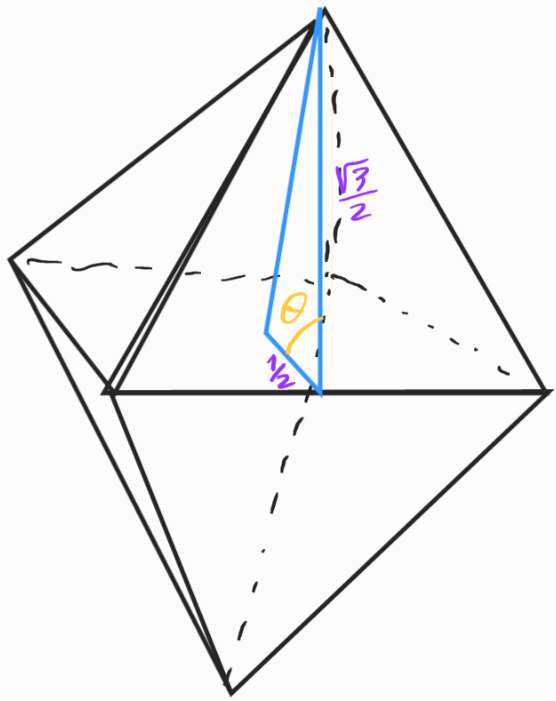
\includegraphics[width=80mm]{imgs/diedral-octaedro}
\end{figure}

Para probar que el cubo $C$ no es equidescomponible con el tetraedro regular $T$ del mismo volumen recurriremos al argumento de Dehn-Hadwiger. Consideramos el $\mathbb{Q}$-espacio vectorial $V$ generado por $\{\pi,\arccos{(1/3)}\}$. Que claramente contiene a los ángulos diedrales del cubo ($\pi/2$) y del tetraedro ($\arccos{(1/3)}$). Supongamos que $\{\pi,\arccos{(1/3)}\}$ es una base de $V$, en ese caso podemos definir una función lineal $f:V\rightarrow\mathbb{R}$ por $f(\pi)=0$ y $f(\arccos{(1/3)})=1$. Como $f$ es lineal y $f(\pi)=0$, también $f(\pi/2)=0$ y $f(C)=12\cdot f(\pi/2)=0$ (el cubo tiene 12 aristas). Como el tetraedro tiene 6 aristas, se tendrá $f(T)=6\cdot f(\arccos{(1/3)})=6$. Como $f(C)\neq f(T)$, $C$ y $T$ no son equidescomponibles.

Este razonamiento funciona siempre que $\{\pi,\arccos{(1/3)}\}$ sea una base de $V$, es claro que es sistema de generadores. Para ver que es linealmente independiente habrá que probar que $\arccos{1/3}$ no puede ser ningún múltiplo racional de $\pi$. Para ello he mirado \href{https://web.math.utk.edu/~jconant/pisol.html}{https://web.math.utk.edu/$\mathtt{\sim}$jconant/pisol.html}.

Supongamos que $\dfrac{\arccos{(1/3)}}{\pi}=\dfrac{p}{q}$ con $p,q$ enteros no nulos. En tal caso % $\displaystyle{e^{i\pi p/q}=e^{i\arccos{(1/3)}}}$
\[e^{i\pi p/q}=e^{i\arccos{(1/3)}}=\frac{1}{3}+\frac{2\sqrt{2}}{3}i,\]
puesto que $\sin\big(\arccos{(1/3)}\big)=\sqrt{1-(1/3)^2}=\sqrt{8}/3$.

Afimamos que 
\[\Big(\frac{1}{3}+\frac{2\sqrt{2}}{3}i\Big)^n=\frac{a_n}{3^{n}}+\frac{b_n\sqrt{2}}{3^{n}}i\]
para algunos enteros $a_n$ y $b_n$. Esto se tiene claramente para $n=1$ con $a_1=1$ y $b_1=2$. Si suponemos que se cumple para $n-1$, tenemos
\begin{align*}
\Big(\frac{1}{3}+\frac{2\sqrt{2}}{3}i\Big)^n&=\Big(\frac{1}{3}+\frac{2\sqrt{2}}{3}i\Big)^{n-1}\Big(\frac{1}{3}+\frac{2\sqrt{2}}{3}i\Big)=\Big(\frac{a_{n-1}}{3^{n-1}}+\frac{b_{n-1}\sqrt{2}}{3^{n-1}}i\Big)\Big(\frac{1}{3}+\frac{2\sqrt{2}}{3}i\Big) \\&=\frac{a_{n-1}}{3^n}-\frac{4b_{n-1}}{3^n}+\frac{2a_{n-1}\sqrt{2}}{3^n}i+\frac{b_{n-1}\sqrt{2}}{3^n}i=\frac{a_{n-1}-4b_{n-1}}{3^n}+\frac{(2a_{n-1}+b_{n-1})\sqrt{2}}{3^n}i
\end{align*}
luego $a_n=a_{n-1}-4b_{n-1}$ y $b_n=b_{n-1}+2a_{n-1}$ son enteros. Ahora probaremos que ningún $b_n$ puede ser 0, en concreto mostraremos que $b_n$ nunca es congruente con 0 en módulo 3: tenemos $a_1=1$, $b_1=2=-1$ (mod 3). Sustituyendo en la recursión obtenemos $a_2=1+4=-1$ y $b_2=-1+2=1$ (mod 3). Sustituyendo una vez más sale $a_3=-1-4=1$ y $b_3=1-2=-1$ (mod 3), por lo que el ciclo se repite y $b_n$ nunca llega a ser un múltiplo de 3.

Finalmente, elevando a $2q$ ambos miembros en la ecuación de las exponenciales llegamos a
\[1=e^{2i\pi p}=\Big(\frac{1}{3}+\frac{2\sqrt{2}}{3}i\Big)^{2q}=\frac{a_{2q}}{3^{2q}}+\frac{b_{2q}\sqrt{2}}{3^{2q}}i,\]
lo cual es absurdo, puesto que $b_{2q}\neq 0$. Concluimos que $\dfrac{\arccos{(1/3)}}{\pi}$ es irracional y $\{\pi,\arccos{(1/3)}\}$ es una base de $V$.

\end{document}

